\documentclass{article}
\usepackage{array}
\newcolumntype{L}{>{\centering\arraybackslash}m{4cm}}
\usepackage[czech]{babel}
\usepackage[utf8]{inputenc}
\usepackage[unicode]{hyperref}
\usepackage{graphicx}
\usepackage{textcomp}
\usepackage[demo]{graphicx}
\usepackage{caption}
\usepackage{subcaption}
\usepackage[T1]{fontenc}
\usepackage[left=2cm, text={17cm, 24cm}, top=2cm]{geometry}
\usepackage[table,xcdraw]{xcolor}
\usepackage{caption}
\usepackage{color}
\usepackage{listings}
\definecolor{mGreen}{rgb}{0,0.6,0}
\definecolor{mGray}{rgb}{0.5,0.5,0.5}
\definecolor{mPurple}{rgb}{0.58,0,0.82}
\definecolor{backgroundColour}{rgb}{0.95,0.95,0.92}
\lstdefinestyle{CStyle}{
    backgroundcolor=\color{backgroundColour},   
    commentstyle=\color{mGreen},
    keywordstyle=\color{magenta},
    numberstyle=\tiny\color{mGray},
    stringstyle=\color{mPurple},
    basicstyle=\footnotesize,
    breakatwhitespace=false,         
    breaklines=true,                 
    captionpos=b,                    
    keepspaces=true,                 
    numbers=left,                    
    numbersep=5pt,                  
    showspaces=false,                
    showstringspaces=false,
    showtabs=false,                  
    tabsize=2,
    language=C
}
\usepackage{hyperref}
\usepackage[sorting=none]{biblatex}
\addbibresource{biblio.bib}
\hypersetup{
    colorlinks=true, % make the links colored
    linkcolor=blue, % color TOC links in blue
    urlcolor=red, % color URLs in red
    linktoc=all % 'all' will create links for everything in the TOC
}

\begin{document}
%%%%%%%%%%%%%%%%%TITULKA%%%%%%%%%%%%%%%%%% 

    \begin{titlepage}
        \begin{center}
            \textsc{\Huge Vysoké Učení Technické v Brně} \\[0.7cm]
            {\Huge Fakulta informačních technologií}
            \center
\includegraphics[width=0.5\linewidth]{./logo.png}\\[5cm]

            \textbf{{\Huge Strojové učení a rozpoznávaní 2020}}\\[0.5cm]

            \textbf{{\huge Dokumentácia k projektu}}\\[0.4cm]
            \LARGE{Detektor jedné osoby z obrázku obličeje a hlasové
nahrávky}\\
            
        \end{center}
        \vfill

        \begin{flushleft}
            \begin{Large}
                \textbf{Marek Žiška}\hspace{44px}\textbf{(xziska03)}\\[0.25cm]
                \textbf{Martin Osvald}\hspace{30px}\textbf{(xosval03)}
            \hfill
            Brno, 30.04.2020
            \end{Large}
        \end{flushleft}

    \end{titlepage}
    \tableofcontents
    \newpage
    \section{Audio systém}
    \subsection{Popis systému}
    \subsubsection{Spracovanie nahrávok}
    \Large{Na vytvorenie systému som použil deep learning knižnicu Keras. Na vyhodnocovanie som sa rozhodol použiť extrakciu príznakov z audio nahrávok. Na extrakciu príznakov som najprv potreboval vyfiltrovať audio nahrávky zo zložiek. Tieto audio nahrávky som načítaval pomocou funkcie \textit{parse\_audio\_files} z jednej zložky \textit{train} v ktorej boli zložky \textit{non\_target} a \textit{target}. Jednotlivé cesty k nahrávkam som si uložil do zoznamu, z ktorého som následne mohol spracovávať jednotlivé nahrávky.}
    \subsubsection{Extrakcia príznakov}
    \Large{Extrakcia prebieha vo funkcií \textit{get\_features}. V tejto časti som dosť experimentoval. Na jednoduchú extrakciu príznakov som použil knižnicu \textit{librosa}. Pri návrhu môjho prvého modelu som z audio nahrávok extrahoval len MFCC príznaky, ktoré mapujú charakteristiky ľudského hlasu. Pri prvom modely som z týchto príznakov vytváral spektogramy, na ktorých som som trénoval konvolučnú neurónovú sieť. Túto metódu som nakoniec ale nepoužil z dôvodu nepresných výsledkov a použil som metódu, v ktorej som si vyextrahované príznaky, názov osoby a nahrávacieho sedenia uložil do csv súbora. Vo funkcií \textit{get\_set\_of\_data} som z csv súbora vytvoril dátové sety: \\ \textit{Train\_data} - numpy pole reprezentujúcé príznaky nahrávok pre dané osoby. Jednotlivé príznaky som s \textit{StandardScaler} vyštandardizoval aby boli dáta viac menej normálovo distribuované a teda znížime možnosť neočakávane zlého natrénovania neúrónovej siete.\\ \textit{Train\_labels} - pole veľkosťou korešpondujúce \textit{Train\_data}, obsahujúce hodnoty 0 pre neznáme osoby a 1 pre hľadanú osobu.\\
    Pri extrakcií a klasifikácií MFCC príznakov som sa ale nedostal k dobrým výsledkom, klasifikátor klasifikoval všetky nahrávky ako neznáme poprípade rozpoznal len zopár cieľových nahrávok. Rozhodol som sa skúsiť rozšíriť trénovací dataset. Rozmýšľal som nad transformáciami nahrávok alebo extrahovaním ďalších príznakov z audio nahrávok. Ako prvé som skúsil extrahovať ďalšie príznaky. Po ktorých pridaní som už dostal rozumnejšie výsledky a k transformáciam nahrávok som sa nedostal. Okrem MFCC som teda skúšal príznaky ako: \\
    Spektrálny centroid - ukazuje na frekvenciu, okolo ktorej je sústredené najvačšie množstvo energie signálu.\\
    Spektrálny rollof - Určuje, kde je uložených 90\% energie spektra.\\
    Spektrálny bandwidth - Ukazuje na rozloženie frekvencie.\\
    Zero crossing rate - Počet prechodov signálu nulou.\\
    Chroma príznak - Indikuje koľko energie je v každej triede tónu.\\
    Postupne som tieto príznaky pridával/kombinoval a najväčšiu presnosť som dosiahol pri zahrnutí všetkých príznakov.
    }
    \subsubsection{Návrh modelov neuronovej siete}
    \Large{Prvý návrh modelu pozostával z dvoch Dense vrstiev, vstupný tvar dát bol počet príznakov extrahovaných z náhravky, aktivačnú funkciu prvej vrstvy som zvolil \textit{relu.} s tým že výstupnú dimenzionalitu som zvolil na 32, druhá vrstva používala aktivačnú funkciu \textit{softmax}, ktorý sa typicky používa pre koncové vrstvy. Výstupná dimenzionalita bola 2, keďže klasifikátor rozdeloval dve triedy(target/non\_target). Model som kompiloval s optimalizačnou funkciou \textit{adam}, ktorý funguje na princípe stochastického poklesu gradientu a je nenáročný na výkon. Loss funkciu som zvolil \textit{sparse\_categorical\_crossentropy}, ktorá je vhodná pre systémy s dvoma a viac výslednými triedami. Pri trénovaní modelu som sa viedol tým že počet epôch budem optimalizovať tak aby sedeli na práve taký počet, kedy sa presnosť modelu na trénovacích dátach blížil k jednej. Bolo to hlavne z dôvodu aby sa model nepretrénoval. Tento model avšak nepriniesol žiadne dobré výsledky, všetky nahrávky označoval za neznáme. Následne som skúšal zvyšovať počet skrytých vrstiev v návrhu modelu a to v takom zmysle aby počty výstupných dimenzionalít regresívne klesali. Taktiež som pri trénovaní zaviedol validačný set dát a všimol som si že, model už dávať presnejšie výsledky.  Pri týchto obmenách som sa dopracoval až k výslednému modelu, z ktorého presnosťou som bol uspokojený. }
    \subsubsection{Generovanie výsledkov}
    \Large{Pri generovaní výsledkov som použil funkcie:\\
    \textit{model.predict\_classes} - ktorá vrátila tvrdé rozhodnutie 0 alebo 1 podľa veľkosti apriórnych pravdepodobností tried\\
    \textit{mode.predict\_proba} - vráti tuple apriórnych pravdepodobností pre každú triedu. Z týchto pravdepodobností som generoval skóre. Skóre teda predstavovalo s akou pravdepodobnosťou si je systém istý tvrdým rozhodnutím. \\
    A z týchto dát som vytvoril požadovaný finálny formát. }
    \subsubsection{Čo by som zmenil}
    \Large{Pri trénovaní by som skúsil nahrávky transformovať a vygenerovať tak viacero nahrávok najmä pre hľadanú osobu, aby sa počty nahrávok pre jednotlivé triedy mierne vyrovnali. Pri trénovaní by sa model natrénoval presnejšie, plus validačný set by dával väčší zmysel, keďže zastúpenie oboch tried by v ňom bolo väčšie nie ako to je v prípade odovzdaného systému, kde pri trénovaní prevažovala trieda \textit{non\_target}. }
 
    \subsection{Návod na zreprodukovanie výsledkov.}
    \Large{Ako prvé je samozrejme potrebné nainštalovanie všetkých nástrojov, uvedených v README. Pre trénovanie bude potrebné vytvoriť zložku \textit{train}, v ktorej budú dve zložky \textit{non\_target} a \textit{target}. V zložkách sú obrázky a nahrávky nehľadaných a hľadanej osoby, na týchto dátach bude systém natrénovaný. Zložku s vyhodnocovacími/nevidenými dátami. \textit{eval}. Trénovanie neurónovej siete som vykonával v jupyter notebooku \textit{audio\_classifier\_MLP.ipynb}. Keďže pri trénovaní neurónovej siete vznikajú rôzne váhy, preto som model na ktorom sa vyhodnocovali evaluačné dáta uložil separátne, aby bolo možné totožné zreprodukovanie výsledkov(súbor \textit{audio\_classifier\_MLP.py}).}
    \newpage
    \section{Image systém}
    \subsection{Popis systému - image\_classificator\_training.py}
    \Large{Program načíta obrázky pomocou png2fea ktorá je upravená z IKRLIB.\\
Png2fea() otvorí obrázok, zmení mu farbu z knižnice cv2 na COLOR\_BGR2GRAY a resizne na dimenziu (80,80). Ked sa resizne tak pomocou imutils zvýrazni hrany. Takýto obrázok potom pridá do slovníka ktorý vráti všetky takto upravené obrázky. \\
    Evaluate()  prechádza obrázky v slovníku   extrahuje príznaky Histogramu Orientovaných Gradientov ( HOG ) z obrázku. Kvôli veľmi malému množstvu obrázkov potom obrázok  točí do + 90 stupňov a do – 90 stupňov a znova extrahuje príznaky  HOG.  V súbore config.json sa dá upraviť cesta z ktorej zložky sa budú načítavať obrázky ako aj options HOG gradientu a ako aj flag na print. Flag print ak je nastavený na 1 tak nám ukazuje ako narába s obrázkami v Evaluate .
}
    \center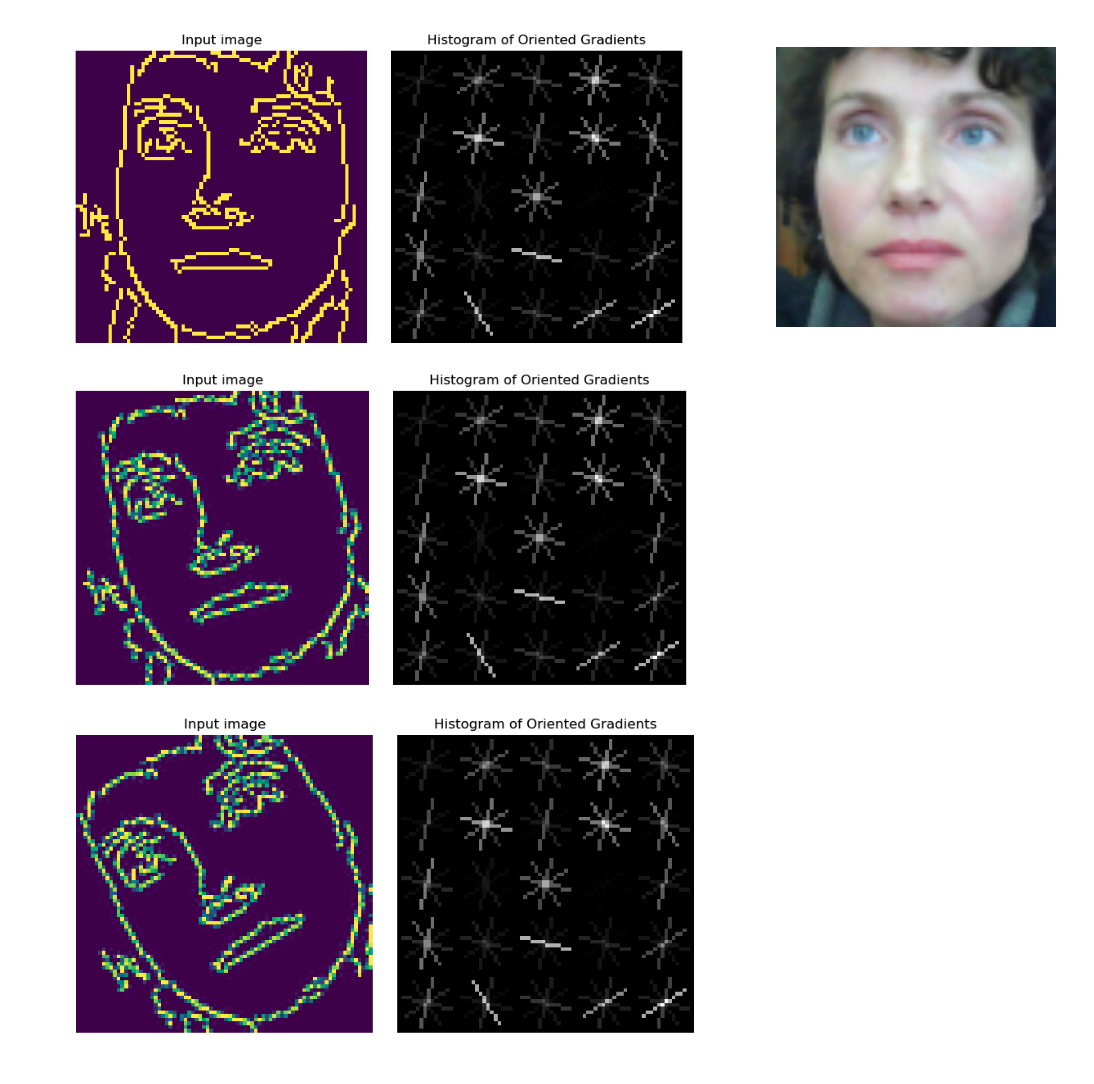
\includegraphics[width=0.85\linewidth]{./image4.png}\\
    \newpage
    \begin{flushleft}
    \Large{HOG funguje na princípe že obrázok  rozdelí do jednotlivých takzvaných cells ( mriežok )  Toto číslo sa dá tiež upraviť v config.json file pod premenou  pixels_per_cell , cell\_per\_block znamena kolko štvorčekom prejdem v rámci blocku.}
    \end{flushleft}

    \center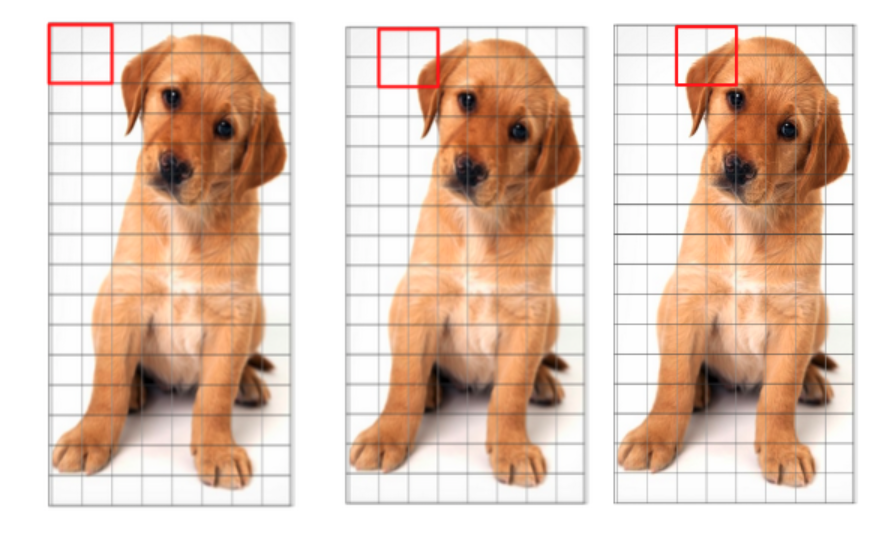
\includegraphics[width=0.9\linewidth]{./image2.png}\\
    \begin{flushleft}
    \Large{V rámci týchto cellov   sa zistí rozdiel medzi jednotlivými pixelmi a podla toho sa určí smer vektoru. 
Za nás to robí funckia HOG ktorá nam vráti array príznakov . }
\end{flushleft}

\center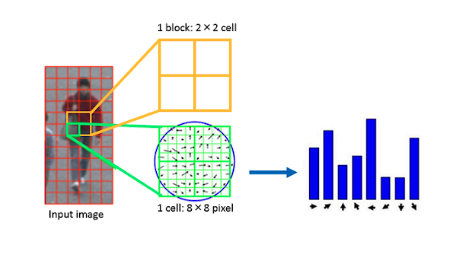
\includegraphics[width=0.9\linewidth]{./image3.png}\\
\center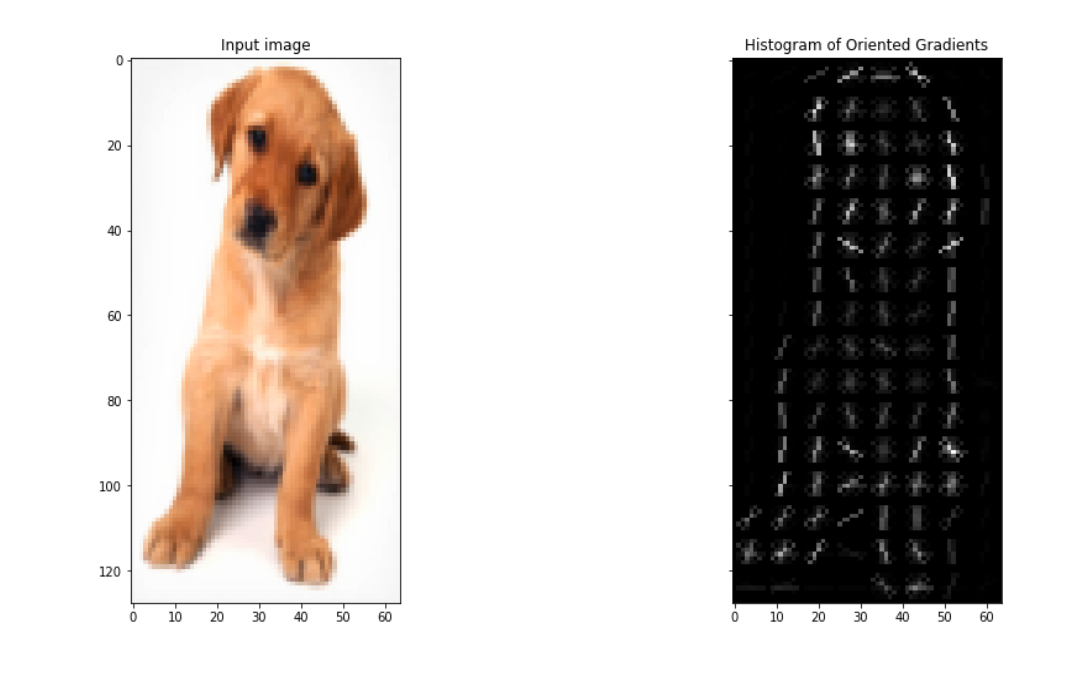
\includegraphics[width=0.9\linewidth]{./image1.png}\\
\begin{flushleft}
\Large{Ku príznakom pridávame ďalší vektor a to buď 1 alebo 0 poďla toho či sme dali non\_target\_train obrázok alebo target\_train. Tieto príznaky  s označením potom trénujeme v Supporteddvector machine  svc ktorá je lineárna. }
\end{flushleft}

\center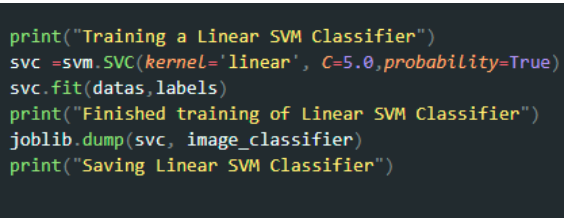
\includegraphics[width=0.9\linewidth]{./image5.png}\\
\begin{flushleft}
\Large{Trénovanie je veľmi rýchle kvôli tomu že  do hog features dávame len dvojfarebné obrázky a rozdelili sme ho na málo blockov.\\   Testovaním sa presnosť zlepšila ak cells\_per\_block dáme menšie čislo kvôli tomu že ak hog gradient vytiahne viac príznakov ako je na obrázku dole  tak klasifikátor potom skoro vždy nevedel určiť či sa daná osoba je na obrázku. Je to kvôoli tomu ,že  by tam bolo o dosť viac hrán a tým pádom aj väčšia nepresnosť.  }
\end{flushleft}

\center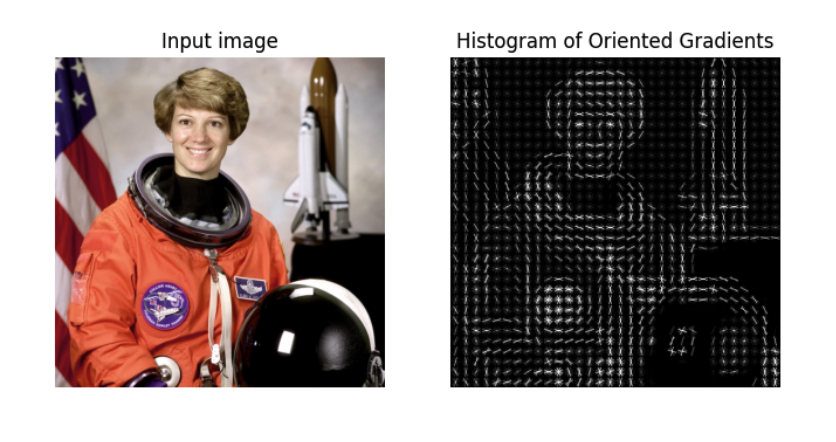
\includegraphics[width=0.9\linewidth]{./image6.png}\\
    \begin{flushleft}

\Large{SVM  nám dokáže oddeliť dve skupiny bodov pomocou nejakého vectoru . SVM využívame na rozdelnie či na obrázku je daný target alebo není .}
\end{flushleft}

\center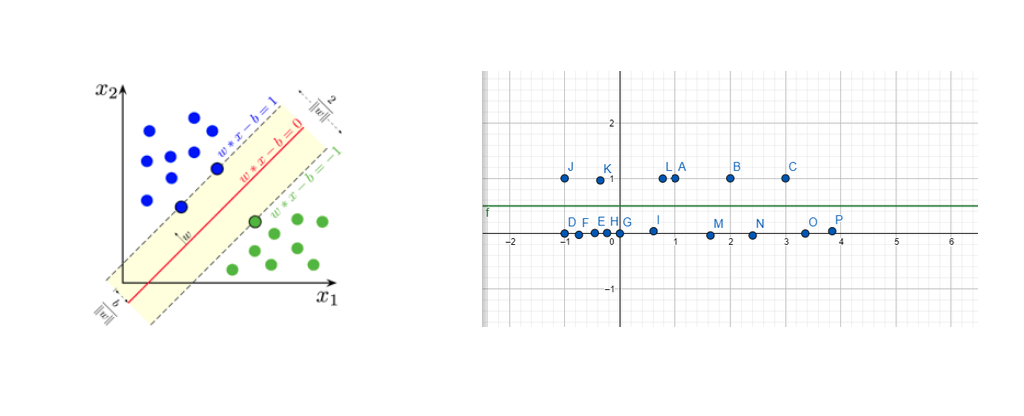
\includegraphics[width=0.9\linewidth]{./image7.png}\\
\subsection{image\_classifier\_evaluation.py}
\begin{flushleft}
\Large{
Znova prechádza  obrázky a otvára ich spôsobom ako v pri trenovaní . ( Otvorí , zmení farbu , resizne na (80,80) a zvýrazni hrany ) Potom extrahuje hog features rovnako ako pri trénovaní a tým že obrázok má rovnakú veľkosť tak nerieši scaling. \\

Score sa zistí pomocou  tohto kódu , kde nastavíme hranu na 0.29 precent. Predict\_proba nám dáva dva výsledky a to percentuálne ako si je istý či to je a či to není daný target.  Pravdepodobne toto zohralo rolu na Cdet.  Snažil som sa vyhovieť požiadavke čim som si viac istejši skóre  , takže keď je rozhodnutie 0 dávam prvé percentá ak je 1 dávam druhé precentá .
}
\subsection{Čo by sa dalo zlepšiť}
\Large{V image klasifikátore sa dali upraviť parametre hog na optimálnu veľkosť príznakov z HOG , teraz sa asi menej príznakov hľadá ako by sa malo. Taktiež by sa dal zväčšiť dataset  pomocou scalingom obrázkov. Vyhodnocovanie klasifikátoru pri obrázkov by taktiež vyhodnocovalo pomocou roznych velkosťí obrázku tak ako sa to robí klasicky podľa hog klasifikátoru. Poprípadne by sa dalo ešte z obrázku najprv vyrezať tvár pomocou univerzálneho predtrénovaného klasifikátoru na tváre , resiznuť pootáčať a natrénovať neuronovú sieť.  Taktiež na nontarget by sa dal zväčšiť dataset pomocou obrázkov z internetu. }
\end{flushleft}
\center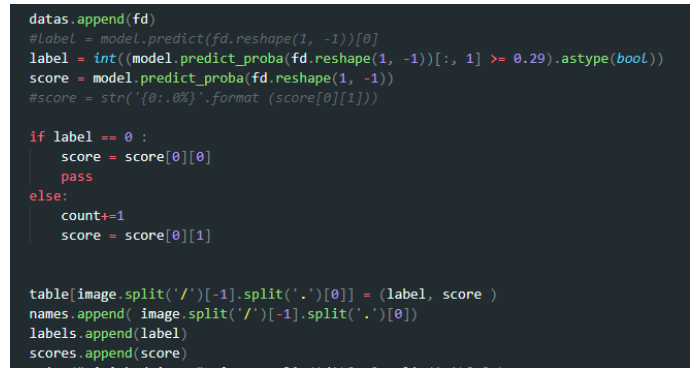
\includegraphics[width=0.9\linewidth]{./image8.png}\\
\newpage
\begin{flushleft}
\section{Image a Audio systém}
\subsection{Popis systému}
\Large{V súbore both.py sa prechádzajú  súbory postupne tak ako v audio klasifikátore tak aj v image klasifikátore. Zistí sa percentuálne score a ako aj tvrdé rozhodnutie obidvoch klasifikátorov. Ak tvrdý výsledok je rovnaký u obidvoch klasifikátorov  tak sa robí aritmetický priemer obidvoch klasifikátorov. Audio klasifikátor bol podľa testovanie presnejší oproti obrázkovému klasifikátoru tak sme mu dali väčšiu váhu. Ak sa score líšili viac ako o 25 percent tak sme sa rozhodovali poďla toho ktorý klasifikátor bol istejší vo výsledku. }
\end{flushleft}
\center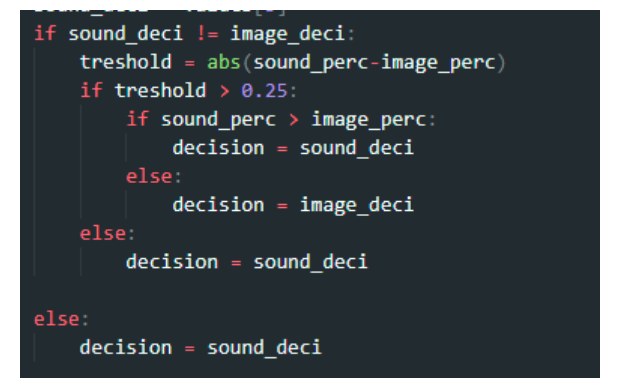
\includegraphics[width=0.9\linewidth]{./image9.png}\\
\end{document}
